%!TEX root=SpGEMM_ACCUMULO_HPEC.tex

\section{TableMult Design}
\label{sDesign}


\subsection{Matrix Multiplication}
\label{sMatMul}
Given matrices $\matr{A}$ of size $N \times M$, $\matr{B}$ of size $M \times L$,
and operations $\oplus$ and $\otimes$ for elementwise addition and multiplication,
the matrix product $\matr{C} = \matr{A} \,{\oplus}.{\otimes}\, \matr{B} $, or more shortly $\matr{C} = \matr{A}\matr{B}$,
defines entries of result matrix $\matr{C}$ as 
\[ \matr{C}(i,j) = \bigoplus_{k=1}^M \matr{A}(i,k) \otimes \matr{B}(k,j) \]
We call intermediary results of $\otimes$ operations \emph{partial products}.

In the case of sparse matrices, we only perform $\oplus$ and $\otimes$ where both operands are nonzero,
an optimization stemming from requiring that 0 is an additive identity of $\oplus$ such that $a \oplus 0 = 0 \oplus a = a$,
and that 0 is a multiplicative annhilator of $\otimes$ such that $a \otimes 0 = 0 \otimes a = 0$.
Sparse arithmetic requires these conditions, because otherwise zero operands could generate nonzero results.

% In Accumulo, zero elements are entries that do not exist in a table. Entries that actually contain the value zero may exist
% from an operation producing a zero value (such as summing partial products 5, -3 and -2).  
% We currently deliver no special treatment to these entries and plan on adding
% an optional feature that removes them when encountered.


We study two well known patterns for computing matrix multiplication:
inner-product and outer-product \cite{kruskal1989techniques}. They differ in the order in which they perform
the $\otimes$ and $\oplus$ operations.  The more common inner-product approach computes each
$\matr{C}(i,j)$ at once by computing the product of the row vector $\matr{A}(i,:)$ with
the column vector $\matr{B}(:,j)$

\removelatexerror
\begin{algorithm}[H]
\vspace{\algspace}
\SetKwBlock{fore}{for}{} 
\SetKw{emit}{emit}
\fore($i = 1\col N$){
\fore($j = 1\col L$){
\emit{$\matr{A}(i,:)  \matr{B}(:,j)$}
}}
\vspace{\algspace}
\end{algorithm}

%\noindent %deferring the inner product's summation, %operation $\cdot$ is inner (also called dot) product on vectors, 
\todo{It is not desirable to defer $\oplus$ because it means we write more individual entries to C.}
In a database context where it is desirable to to defer additions to be performed by the output table $\matr{C}$ (using Accumulo's builtin summing combiners), the above approach can be rewritten as

\removelatexerror
\begin{algorithm}[H]
\vspace{\algspace}
\SetKwBlock{fore}{for}{} 
\SetKw{emit}{emit}
\fore($i = 1\col N$){
\fore($j = 1\col L$){
\fore($k = 1\col M$){
\emit{$\matr{A}(i,k) \otimes \matr{B}(k,j)$}
}}}
\vspace{\algspace}
\end{algorithm}

The inner-product has the advantage of generating entries in sorted order.  All partial products needed 
to compute a particular element $\matr{C}(i,j)$ are generated consecutively by the third-level loop.
The $\oplus$ is applied immediately after each third-level loop to obtain an element in $\matr{C}$.
The inner-product is easy to ``pre-sum,'' an Accumulo term for applying a Combiner
locally before sending entries to a remote but globally-aware table combiner.
% move to another section?
%Inner product also generates output ``in order'' in a second sense: 
Emitting sorted entries also allows inner product to be used in standard iterator stacks.
%% It is also adventageous that inner product generates entries sorted by row 
%% and column, which allows inner product to be used in standard iterator stacks that require sorted output.

Despite its order-preserving advantages, an outer-product algorithm performs better for sparse matrices 
because it requires on one pass of the data \cite{burkhardt2013big}\cite{burkhardt2014asking}.  The inner-product requires repeating
the second-level loop that scans over all of $\matr{B}$.
%The same effect holds if we flipped the process symmetrically.
Under our assumption that we cannot fit $\matr{B}$ entirely in memory,
multiple passes over $\matr{B}$ translates to multiple Accumulo scans that each require a disk read.
We found in performance tests that an outer-product approach performed an order-of-magnitude better than an inner-product approach.
%multiple scans over $\matr{B}$ 
%performed an order of magnitude worse, taking over 100 seconds to multiply SCALE 11 inputs 
%(see Section~\ref{sPerformance})
%whereas an outer product method ran in under 8.

Outer product matrix multiply runs the following

\removelatexerror
\begin{algorithm}[H]
\vspace{\algspace}
\SetKwBlock{fore}{for}{} 
\SetKw{emit}{emit}
\fore($k = 1\col M$){
\emit{$\matr{A}(:,k) \matr{B}(k,:)$}
}
\vspace{\algspace}
\end{algorithm}

\noindent %deferring outer product's summation, which we unfold as %where the operation $\times$ is outer (also called tensor or Carteisan) product on vectors, which we may unfold as
performing outer %(also called tensor or Cartesian) 
product
on vectors, 
which we unfold as

\removelatexerror
\begin{algorithm}[H]
\vspace{\algspace}
\SetKwBlock{fore}{for}{} 
\SetKw{emit}{emit}
\fore($k = 1\col M$){
\fore($i = 1\col N$){
\fore($j = 1\col L$){
\emit{$ \matr{A}(i,k) \otimes \matr{B}(k,j)$}
}}}
\vspace{\algspace}
\end{algorithm}

Outer product emits partial products in unsorted order.
This is due to moving the $i$ and $j$ loops
that determine partial product position
below the top-level $k$ loop.

On the other hand, outer product only requires a single pass over both input matrices.
This is because the top-level $k$ loop fixes a dimension of both $\matr{A}$ and $\matr{B}$.
Once we finish processing a column of $\matr{A}$ and row of $\matr{B}$,
we never need read them again.% (i.e., we never need to restart the top-level $k$ loop).

In terms of memory usage, outer product works best when either the matching row or column fits in memory.
If neither fits, then we could run the algorithm 
with a ``no memory assumption'' streaming approach
by re-reading $\matr{B}$'s rows while streaming through $\matr{A}$'s columns 
(or vice versa by symmetry of $i$ and $j$),
perhaps at the cost of extra disk reads.
%% %as suggested by the second-level loop repeating the third-level loop running through rows of $\matr{B}$.
%% %Storing one row in memory is a much lower cost than storing a whole matrix in memory.
%% We may implement the ``no memory assumption'' streaming approach in Accumulo by using
%% deepCopy SKVI methods to store ``pointers'' to the beginning of $\matr{B}$'s rows
%% (or $\matr{A}$'s columns),
%% perhaps at the cost of extra disk reads.
%% %However, this strategy may come at the cost of extra disk seeks, and so
%% %we leave testing its performance to future work, for now storing the current row of table $\matr{B}$ in memory.

Because $k$ runs along $\matr{A}$'s second dimension 
and Accumulo uses row-oriented data layouts, we implement 
TableMult to operate on $\matr{A}$'s transpose $\matr{A^\tr}$.



\subsection{TableMult Iterators}
\label{sTableMult}

We implement SpGEMM with three iterators placed on a BatchScan of table $\matr{B}$:
RemoteSourceIterator, TwoTableIterator and RemoteWriteIterator.
The BatchScanner directs Accumulo to run the iterators on tablets of $\matr{B}$ in parallel.
%The: We place these iterators on  scan itself emits no entries except for a smidgeon of ``monitoring entries'' 
%that inform the client about TableMult progress. 
%% Instead, the scan on table $\matr{B}$ reads from table $\matr{A}$T
%% by opening a Scanner and writes to result table $\matr{C}$
%% by opening a BatchWriter, all within the scan's iterator stack.
%% See Figure~\ref{fIteratorStackSpGEMM} for an illustration.

The key idea behind the TableMult iterators is that they divert normal dataflow by opening a BatchWriter,
%reducing entries sent to the client to zero and instead sending 
redirecting entries out-of-band to $\matr{C}$ via
Accumulo's ingest channel that does not require sorted order. 
The scan itself emits no entries except for a small number of ``monitoring entries'' 
that inform the client about TableMult progress.
%Thus the TableMult iterators act as reduction iterators, even though they actually transmit 
%a huge stream of entries out-of-band to another Accumulo table.
We enable multi-table iterator dataflow by opening Scanners 
that read remote Accumulo tables out-of-band.
%which in the case of SpGEMM means scanning table $\matr{A^\tr}$.
Scanners and BatchWriters are standard tools for Accumulo clients; 
by creating them inside iterators, we enable client-side processing patterns
within tablet servers.

We illustrate TableMult's data flow in Figure~\ref{fIteratorStackSpGEMM},
placing a Scanner on table $\matr{A^\tr}$
and a BatchWriter on result table $\matr{C}$.

\begin{figure}[htb]
\vspace{-3pt}
\centering
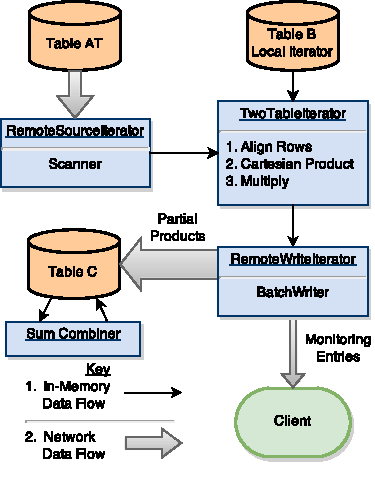
\includegraphics[width=3.0in]{TableMultIteratorStack}
\vspace{-8pt}
\caption{Data flow through the TableMult iterator stack}
\label{fIteratorStackSpGEMM}
\vspace{-9pt}
\end{figure}

\subsubsection{RemoteSourceIterator}
RemoteSourceIterator scans an Accumulo table
(not necessarily in the same cluster) %with the same range it is seeked to
%using credentials from the client.
using credentials passed from the client through iterator options.
%Clients pass connection information through iterator options.
%% Clients pass connection information including zookeeper hosts, timeout,
%% username and password via iterator options. %in the form of a \texttt{Map<String,String>}.
%% We leave more secure scan authentication methods to future work,
%% although only users with access to the Accumulo instance may see the password in iterator options.

We also use iterator options to specify row and column subsets, 
encoding them in a string format similar to that in D4M \cite{kepner2012dynamic}.
Row subsets are straightforward since Accumulo uses row-oriented indexing.
Column subsets can be implemented with filter iterators
but do not improve performance since Accumulo must read every column from disk.
We encourage users to maintain a tranpose table
using strategies similiar to the D4M Schema \cite{kepner2013d4m}
for cases requiring column indexing.

Multiplying table subsets is crucial for queued analytics on selected rows.
However for simpler performance evaluation, 
our experiments in Section~\ref{sPerformance} multiply whole tables.

\subsubsection{TwoTableIterator}
TwoTableIterator reads from two iterator sources, one for $\matr{A^\tr}$ and one for $\matr{B}$,
and performs the core operations of the outer product algorithm in three phases:
\begin{enumerate}
\item Align Rows.  Read entries from $\matr{A^\tr}$ and $\matr{B}$ until they advance to a matching row
or one runs out of entries. We skip non-matching rows 
since they would multiply with an all-zero row that, by Section~\ref{sMatMul}'s assumptions,
generate all zero patrial products.
\item Cartesian product. Read both matching rows into an in-memory data structure. 
Initialize an iterator that emits pairs of entries from the rows' Cartesian product.
\item Multiply. Pass pairs of entries to $\otimes$ and emit results. 
\end{enumerate}

A client defines $\otimes$ by specifying a class 
that implements a provided ``multiply interface.''
%which TwoTableIterator instantiates and calls. 
For our experiments we implement $\otimes$ as java.math.BigDecimal multiplication
which guarantees correctness under large or precise real numbers.
BigDecimal decoding did not noticeably impact performance.

\subsubsection{RemoteWriteIterator}
RemoteWriteIterator writes entries to a remote Accumulo table using a BatchWriter. %created on \texttt{init}.
Entries do not have to be in sorted order because Accumulo sorts incoming entries as part of its
 ingest process. 
%% Like RemoteSourceIterator, the client passes connection information 
%% for the remote table via iterator options.

Barring extreme events such as exceptions in the iterator stack or thread death,
we designed RemoteWriteIterator to maintain correctness, such that entries generated from
its source write to the remote table once.
We accomplish this by performing all BatchWriter operations within a single function call
before ceding thread control back to the tablet server.  

A performance concern remains when multiplying a subset of the input tables' rows 
that consists of many disjoint ranges, such as one million ``singleton'' ranges spanning one row each.
It is inefficient to flush the BatchWriter before returning from each seek call, which happens once per 
disjoint scan range. %, and a known Accumulo issue could even crash the tablet server \cite{ACCUMULO-3710}.
We accomodate this case by ``transferring seek control'' %over desired row range subsets
from the tablet server to RemoteWriteIterator 
via the same strategy used in RemoteSourceIterator for seeking within an iterator.
%by encoding range objects in iterator options. %using the same technique RemoteSourceIterator uses, 
%% as opposed to the usual method of 
%% passing range objects to the %\texttt{setRanges} 
%% BatchScanner on $\matr{B}$.
%% %% RemoteWriteIterator traverses all ranges in the desired subset 
%% %% (within the tablet it runs on) in one call to seek.
%% %% %In the case of multiple tablets for table $\matr{B}$, RemoteWriteIterator running on each tablet handles 
%% %% %the portion of ranges that intersects with the range of keys in its tablet.

We include an option to BatchWrite $\matr{C}$'s transpose $\matr{C^\tr}$ in place of or alongside $\matr{C}$. 
Writing $\matr{C^\tr}$ facilitates chaining TableMults together
and maintenance of transpose indexing.

\subsubsection{Lazy $\oplus$}
We lazily sum partial products by placing a Combiner subclass implementing BigDecimal addition 
on table $\matr{C}$ at scan, minor and major compaction scopes.
Thus, $\oplus$ occurs sometime after RemoteWriteIterator writes partial products to $\matr{C}$
yet necessarily before entries from $\matr{C}$ may be seen such that we always achieve correctness.
Summation could happen when Accumulo flushes table $\matr{C}$'s entries cached in memory to a new RFile, 
when Accumulo compacts RFiles together, or when a client scans $\matr{C}$. 

The key algebraic requirement for implementing $\oplus$ inside a Combiner
is that $\oplus$ must be associative and commutative.
These properties allow us to apply $\oplus$ to subsets of a result element's partial products 
and to any ordering of them, which is chaotic by outer product's nature.
If we truly had an $\oplus$ operation that required seeing all partial products at once,
we would have to either gather partial products at the client or initiate a full major compaction.

\subsubsection{Monitoring}
RemoteWriteIterator never emits entries to the client by default. 
One downside of this approach is that clients cannot precisely track the progress of a TableMult operation,
which may frustrate users expecting a more interactive computing experience.
Clients could query the Accumulo monitor for read/write rates 
or prematurely scan partial products written to $\matr{C}$, but both approaches are too coarse.
%having only access to coarse Accumulo monitor rate information or partial product scans on $\matr{C}$.
%% The only information clients would have are scan and write rates from the Accumulo monitor,
%% whether a scan is running, idle or queued from the tablet server, and what partial products 
%% are written so far from scanning $\matr{C}$.

We therefore implement a monitoring option that emits a value
containing the number of entries TwoTableIterator processed
at a client-set frequency.
RemoteWriteIterator emits monitoring entries at ``safe'' points, that is,
points at which we can recover the iterator stack's state 
if Accumulo destroys, re-creates and re-seeks it.
%to a range starting from its last emitted key.
Stopping after emitting the last value in the outer product of two rows is safe 
because we place the last value's row key in the monitoring key and know, 
in the event of an iterator stack rebuild, to proceed to the next matching row.
We may succeed in stopping during an outer product 
by encoding more information in the monitoring key.
%We are also experimenting with stopping in the middle of an outer product by encoding the 
%column family and qualifier of input tables' keys in the monitoring key.


%%\subsubsection{Client API}
%% The following shows how client programs call TableMult in Java:

%% %\todo[inline]{Put Java signature of TableMult call?}

%% \definecolor{javared}{rgb}{0.6,0,0} % for strings
%% \definecolor{javagreen}{rgb}{0.25,0.5,0.35} % comments
%% \definecolor{javapurple}{rgb}{0.5,0,0.35} % keywords
%% \definecolor{javadocblue}{rgb}{0.25,0.35,0.75} % javadoc
 
%% \lstset{language=Java,
%% basicstyle=\ttfamily,
%% keywordstyle=\color{javapurple}\bfseries,
%% stringstyle=\color{javared},
%% commentstyle=\color{javagreen},
%% morecomment=[s][\color{javadocblue}]{/**}{*/},
%% numbers=left,
%% numberstyle=\tiny\color{black},
%% stepnumber=2,
%% numbersep=10pt,
%% tabsize=4,
%% showspaces=false,
%% showstringspaces=false}

%% \begin{lstlisting}

%% \end{lstlisting}

